%%%%%%%%%%%%%%%%%%%%%%%%%%%%%%%%%%%%%%%%%%%%%%%%%%%%%%%%%%%%%%%%%%%%%%%%%%%%%%%%
%%%%%%%%%%%%%%%%%%%%%%%%%%%%%%%%%%%%%%%%%%%%%%%%%%%%%%%%%%%%%%%%%%%%%%%%%%%%%%%%
%%                                                                            %%
%% thesistemplate.tex version 3.20 (2018/08/31)                               %%
%% The LaTeX template file to be used with the aaltothesis.sty (version 3.20) %%
%% style file.                                                                %%
%% This package requires pdfx.sty v. 1.5.84 (2017/05/18) or newer.            %%
%%                                                                            %%
%% This is licensed under the terms of the MIT license below.                 %%
%%                                                                            %%
%% Written by Luis R.J. Costa.                                                %%
%% Currently developed at the Learning Services of Aalto University School of %%
%% Electrical Engineering by Luis R.J. Costa since May 2017.                  %%
%%                                                                            %%
%% Copyright 2017-2018, by Luis R.J. Costa, luis.costa@aalto.fi,              %%
%% Copyright 2017-2018 Swedish translations in aaltothesis.cls by Elisabeth   %%
%% Nyberg, elisabeth.nyberg@aalto.fi and Henrik Wallén,                       %%
%% henrik.wallen@aalto.fi.                                                    %%
%% Copyright 2017-2018 Finnish documentation in the template opinnatepohja.tex%%
%% by Perttu Puska, perttu.puska@aalto.fi, and Luis R.J. Costa.               %%
%% Copyright 2018 English template thesistemplate.tex by Luis R.J. Costa.     %%
%% Copyright 2018 Swedish template kandidatarbetsbotten.tex by Henrik Wallen. %%
%%                                                                            %%
%% Permission is hereby granted, free of charge, to any person obtaining a    %%
%% copy of this software and associated documentation files (the "Software"), %%
%% to deal in the Software without restriction, including without limitation  %%
%% the rights to use, copy, modify, merge, publish, distribute, sublicense,   %%
%% and/or sell copies of the Software, and to permit persons to whom the      %%
%% Software is furnished to do so, subject to the following conditions:       %%
%% The above copyright notice and this permission notice shall be included in %%
%% all copies or substantial portions of the Software.                        %%
%% THE SOFTWARE IS PROVIDED "AS IS", WITHOUT WARRANTY OF ANY KIND, EXPRESS OR %%
%% IMPLIED, INCLUDING BUT NOT LIMITED TO THE WARRANTIES OF MERCHANTABILITY,   %%
%% FITNESS FOR A PARTICULAR PURPOSE AND NONINFRINGEMENT. IN NO EVENT SHALL    %%
%% THE AUTHORS OR COPYRIGHT HOLDERS BE LIABLE FOR ANY CLAIM, DAMAGES OR OTHER %%
%% LIABILITY, WHETHER IN AN ACTION OF CONTRACT, TORT OR OTHERWISE, ARISING    %%
%% FROM, OUT OF OR IN CONNECTION WITH THE SOFTWARE OR THE USE OR OTHER        %%
%% DEALINGS IN THE SOFTWARE.                                                  %%
%%                                                                            %%
%%                                                                            %%
%%%%%%%%%%%%%%%%%%%%%%%%%%%%%%%%%%%%%%%%%%%%%%%%%%%%%%%%%%%%%%%%%%%%%%%%%%%%%%%%
%%                                                                            %%
%%                                                                            %%
%% An example for writting your thesis using LaTeX                            %%
%% Original version and development work by Luis Costa, changes to the text   %% 
%% in the Finnish template by Perttu Puska.                                   %%
%% Support for Swedish added 15092014                                         %%
%% PDF/A-b support added on 15092017                                          %%
%% PDF/A-2 support added on 24042018                                          %%
%%                                                                            %%
%% This example consists of the files                                         %%
%%         thesistemplate.tex (version 3.20) (for text in English)            %%
%%         opinnaytepohja.tex (version 3.20) (for text in Finnish)            %%
%%         kandidatarbetsbotten.tex (version 1.00) (for text in Swedish)      %%
%%         aaltothesis.cls (versio 3.20)                                      %%
%%         kuva1.eps (graphics file)                                          %%
%%         kuva2.eps (graphics file)                                          %%
%%         kuva1.jpg (graphics file)                                          %%
%%         kuva2.jpg (graphics file)                                          %%
%%         kuva1.png (graphics file)                                          %%
%%         kuva2.png (graphics file)                                          %%
%%         kuva1.pdf (graphics file)                                          %%
%%         kuva2.pdf (graphics file)                                          %%
%%                                                                            %%
%%                                                                            %%
%% Typeset in Linux either with                                               %%
%% pdflatex: (recommended method)                                             %%
%%             $ pdflatex thesistemplate                                      %%
%%             $ pdflatex thesistemplate                                      %%
%%                                                                            %%
%%   The result is the file thesistemplate.pdf that is PDF/A compliant, if    %%
%%   you have chosen the proper \documenclass options (see comments below)    %%
%%   and your included graphics files have no problems.
%%                                                                            %%
%% Or                                                                         %%
%% latex: (this method is not recommended)                                    %%
%%             $ latex thesistemplate                                         %%
%%             $ latex thesistemplate                                         %%
%%                                                                            %%
%%   The result is the file thesistemplate.dvi, which is converted to ps      %%
%%   format as follows:                                                       %%
%%                                                                            %%
%%             $ dvips thesistemplate -o                                      %%
%%                                                                            %%
%%   and then to pdf as follows:                                              %%
%%                                                                            %%
%%             $ ps2pdf thesistemplate.ps                                     %%
%%                                                                            %%
%%   This pdf file is not PDF/A compliant. You must must make it so using,    %%
%%   e.g., Acrobat Pro or PDF-XChange.                                        %%
%%                                                                            %%
%%                                                                            %%
%% Explanatory comments in this example begin with the characters %%, and     %%
%% changes that the user can make with the character %                        %%
%%                                                                            %%
%%%%%%%%%%%%%%%%%%%%%%%%%%%%%%%%%%%%%%%%%%%%%%%%%%%%%%%%%%%%%%%%%%%%%%%%%%%%%%%%
%%%%%%%%%%%%%%%%%%%%%%%%%%%%%%%%%%%%%%%%%%%%%%%%%%%%%%%%%%%%%%%%%%%%%%%%%%%%%%%%
%%
%% WHAT is PDF/A
%%
%% PDF/A is the ISO-standardized version of the pdf. The standard's goal is to
%% ensure that he file is reproducable even after a long time. PDF/A differs
%% from pdf in that it allows only those pdf features that support long-term
%% archiving of a file. For example, PDF/A requires that all used fonts are
%% embedded in the file, whereas a normal pdf can contain only a link to the
%% fonts in the system of the reader of the file. PDF/A also requires, among
%% other things, data on colour definition and the encryption used.
%% Currently three PDF/A standards exist:
%% PDF/A-1: based on PDF 1.4, standard ISO19005-1, published in 2005.
%%          Includes all the requirements essential for long-term archiving.
%% PDF/A-2: based on PDF 1.7, standard ISO19005-2, published in 2011.
%%          In addition to the above, it supports embedding of OpenType fonts,
%%          transparency in the colour definition and digital signatures.
%% PDF/A-3: based on PDF 1.7, standard ISO19005-3, published in 2012.
%%          Differs from the above only in that it allows embedding of files in
%%          any format (e.g., xml, csv, cad, spreadsheet or wordprocessing
%%          formats) into the pdf file.
%% PDF/A-1 files are not necessarily PDF/A-2 -compatible and PDF/A-2 are not
%% necessarily PDF/A-1 -compatible.
%% All of the above PDF/A standards have two levels:
%% b: (basic) requires that the visual appearance of the document is reliably
%%    reproduceable.
%% a (accessible) in addition to the b-level requirements, specifies how
%%   accessible the pdf file is to assistive software, say, for the physically
%%   impaired.
%% For more details on PDF/A, see, e.g., https://en.wikipedia.org/wiki/PDF/A
%%
%%
%% WHICH PDF/A standard should my thesis conform to?
%%
%% Primarily to the PDF/A-1b standard. All the figures and graphs typically
%% use in thesis work do not require transparency features, a basic '2-D'
%% visualisation suffices. The font to be used are specified in this template
%% and they should not be changed. However, if you have figures where
%% transparency characteristics matter, use the PDF/A-2b standard. Do not use
%% the PDF/A-3b standard for your thesis.
%%
%%
%% WHAT graphics format can I use to produce my PDF/A compliant file?
%%
%% When using pdflatex to compile your work, use jpg, png or pdf files. You may
%% have PDF/A compliance problems with figures in pdf format. Do not use PDF/A
%% compliant graphics files.
%% If you decide to use latex to compile your work, the only acceptable file
%% format for your figure is eps. DO NOT use the ps format for your figures.

%% USE one of these:
%% * the first when using pdflatex, which directly typesets your document in the
%%   chosen pdf/a format and you want to publish your thesis online,

%% * the second when you want to print your thesis to bind it, or
%% * the third when producing a ps file and a pdf/a from it.
%%
\documentclass[english, 12pt, a4paper, sci, utf8, a-1b, online]{aaltothesis}
%\documentclass[english, 12pt, a4paper, elec, utf8, a-1b]{aaltothesis}
%\documentclass[english, 12pt, a4paper, elec, dvips, online]{aaltothesis}

%% Use the following options in the \documentclass macro above:
%% your school: arts, biz, chem, elec, eng, sci
%% the character encoding scheme used by your editor: utf8, latin1
%% thesis language: english, finnish, swedish
%% make an archiveable PDF/A-1b or PDF/A-2b compliant file: a-1b, a-2b
%%                    (with pdflatex, a normal pdf containing metadata is
%%                     produced without the a-*b option)
%% typeset in symmetric layout and blue hypertext for online publication: online
%%            (no option is the default, resulting in a wide margin on the
%%             binding side of the page and black hypertext)
%% two-sided printing: twoside (default is one-sided printing)
%%

%% Use one of these if you write in Finnish (see the Finnish template
%% opinnaytepohja.tex)
%\documentclass[finnish, 12pt, a4paper, elec, utf8, a-1b, online]{aaltothesis}
%\documentclass[finnish, 12pt, a4paper, elec, utf8, a-1b]{aaltothesis}
%\documentclass[finnish, 12pt, a4paper, elec, dvips, online]{aaltothesis}

\usepackage{graphicx}
\usepackage{tabularx}
\usepackage{float}
\usepackage{caption}

%% Math fonts, symbols, and formatting; these are usually needed
\usepackage{amsfonts,amssymb,amsbsy,amsmath}

% Different bibliography styles can be found from https://www.overleaf.com/learn/latex/Bibtex_bibliography_styles
\usepackage{natbib}
\bibliographystyle{apa}

%% Change the school field to specify your school if the automatically set name
%% is wrong
% \university{aalto-yliopisto}
% \school{Sähkötekniikan korkeakoulu}

%% Edit to conform to your degree programme
%%
\degreeprogram{Computer, Communication and Information Sciences}
%%

%% Your major
%%
\major{Software and Service Engineering}
%%

%% Major subject code
%%
\code{SCI3043}
%%
 
%% Choose one of the three below
%%
%\univdegree{BSc}
\univdegree{MSc}
%\univdegree{Lic}
%%

%% Your name (self explanatory...)
%%
\thesisauthor{Anders Nylund}
%%

%% Your thesis title comes here and possibly again together with the Finnish or
%% Swedish abstract. Do not hyphenate the title, and avoid writing too long a
%% title. Should LaTeX typeset a long title unsatisfactorily, you mght have to
%% force a linebreak using the \\ control characters.
%% In this case...
%% Remember, the title should not be hyphenated!
%% A possible "and" in the title should not be the last word in the line, it
%% begins the next line.
%% Specify the title again without the linebreak characters in the optional
%% argument in box brackets. This is done because the title is part of the 
%% metadata in the pdf/a file, and the metadata cannot contain linebreaks.
%%
\thesistitle{Developer Experience}
%\thesistitle[Title of the thesis]{Title of\\ the thesis}
%%

%%
\place{Espoo}
%%

%% The date for the bachelor's thesis is the day it is presented
%%
\date{TBA}
%%

\newcommand{\now}{autumn 2019}

%% Thesis supervisor
%% Note the "\" character in the title after the period and before the space
%% and the following character string.
%% This is because the period is not the end of a sentence after which a
%% slightly longer space follows, but what is desired is a regular interword
%% space.
%%
\supervisor{Prof.\ Pirjo Professor}
%%

%% Advisor(s)---two at the most---of the thesis. Check with your supervisor how
%% many official advisors you can have.
%%
\advisor{Dr Alan Advisor}
%\advisor{MSc Sarah Scientist}
%%

%% Aaltologo: syntax:
%% \uselogo{aaltoRed|aaltoBlue|aaltoYellow|aaltoGray|aaltoGrayScale}{?|!|''}
%% The logo language is set to be the same as the thesis language.
%%
\uselogo{aaltoRed}{''}
%%

%% The English abstract:
%% All the details (name, title, etc.) on the abstract page appear as specified
%% above.
%% Thesis keywords:
%% Note! The keywords are separated using the \spc macro
%%
\keywords{Developer Experience\spc Software Projects}
%%

%% The abstract text. This text is included in the metadata of the pdf file as well
%% as the abstract page.
%%

\newcommand{\englishabstract}{The abstract in english}
\newcommand{\swedishabstract}{Sammandrag på svenska}

\thesisabstract{
  \englishabstract
}

%% Copyright text. Copyright of a work is with the creator/author of the work
%% regardless of whether the copyright mark is explicitly in the work or not.
%% You may, if you wish, publish your work under a Creative Commons license (see
%% creaticecommons.org), in which case the license text must be visible in the
%% work. Write here the copyright text you want. It is written into the metadata
%% of the pdf file as well.
%% Syntax:
%% \copyrigthtext{metadata text}{text visible on the page}
%% 
%% In the macro below, the text written in the metadata must have a \noexpand
%% macro before the \copyright special character, and macros (\copyright and
%% \year here) must be separated by the \ character (space chacter) from the
%% text that follows. The macros in the argument of the \copyrighttext macro
%% automatically insert the year and the author's name. (Note! \ThesisAuthor is
%% an internal macro of the aaltothesis.cls class file).
%% Of course, the same text could have simply been written as
%% \copyrighttext{Copyright \noexpand\copyright\ 2018 Eddie Engineer}
%% {Copyright \copyright{} 2018 Eddie Engineer}
%%
\copyrighttext{Copyright \noexpand\copyright\ \number\year\ \ThesisAuthor}
{Copyright \copyright{} \number\year{} \ThesisAuthor}

%% You can prevent LaTeX from writing into the xmpdata file (it contains all the 
%% metadata to be written into the pdf file) by setting the writexmpdata switch
%% to 'false'. This allows you to write the metadata in the correct format
%% directly into the file thesistemplate.xmpdata.
%\setboolean{writexmpdatafile}{false}

%% All that is printed on paper starts here
%%
\begin{document}

%% Create the coverpage
%%
\makecoverpage

%% Typeset the copyright text.
%% If you wish, you may leave out the copyright text from the human-readable
%% page of the pdf file. This may seem like a attractive idea for the printed
%% document especially if "Copyright (c) yyyy Eddie Engineer" is the only text
%% on the page. However, the recommendation is to print this copyright text.
%%
\makecopyrightpage

%% Note that when writting your thesis in English, place the English abstract
%% first followed by the possible Finnish or Swedish abstract.

%% Abstract text
%% All the details (name, title, etc.) on the abstract page appear as specified
%% above.
%%
\begin{abstractpage}[english]
  \englishabstract
\end{abstractpage}

%% The text in the \thesisabstract macro is stored in the macro \abstractext, so
%% you can use the text metadata abstract directly as follows:
%%
%\begin{abstractpage}[english]
%	\abstracttext{}
%\end{abstractpage}

%% Force a new page so that the possible Finnish or Swedish abstract does not
%% begin on the same page
%%
% \newpage
% %%
% %% Abstract in Finnish.  Delete if you don't need it. 
% %%
% \thesistitle{Opinnäyteen otsikko}
% \supervisor{Prof.\ Pirjo Professori}
% \advisor{TkT Alan Advisor}
% \degreeprogram{Elektroniikka ja sähkötekniikka}
% %\department{Elektroniikan ja nanotekniikan laitos}
% \major{Sopiva pääaine}
% %% The keywords need not be separated by \spc now.
% \keywords{Vastus, resistanssi, lämpötila}
% %% Abstract text
% \begin{abstractpage}[finnish]
%   Tiivistelmässä on lyhyt selvitys
%   kirjoituksen tärkeimmästä sisällöstä: mitä ja miten on tutkittu,
%   sekä mitä tuloksia on saatu. 
% \end{abstractpage}

%% Force new page so that the Swedish abstract starts from a new page
\newpage

%% Swedish abstract. Delete it if you don't need it. 
%% 
\thesistitle{Developer Experience}
\supervisor{Prof.\ Pirjo Professori}
\advisor{TkD Alan Advisor} %
\degreeprogram{Computer, Communication and Information Sciences}
\department{Institutionen för radiovetenskap och -teknik}%
%% Abstract keywords
\keywords{Nyckelord på svenska, temperatur}
%% Abstract text
\begin{abstractpage}[swedish]
  \swedishabstract
\end{abstractpage}

%% Preface
%%
%% This section is optional. Remove it if you do not want a preface.
\mysection{Preface}
I want to thank everyone so far that has shown interested and been involved in this thesis. Even if the thesis is still in it's early phases, I am surprised of how many have showed interest towards it and offered a helping hand.
\newline \\ After the thesis has been finalized there will probably be many more appreciations to give

\vspace{5cm}
Otaniemi, Date to te announced

\vspace{5mm}
{\hfill Anders Nylund \hspace{1cm}}

%% Force a new page after the preface
%%
\newpage


%% Table of contents. 
%%
\thesistableofcontents

%% Symbols and abbreviations
\mysection{Thesis dictionary}

\begin{tabular}{ll}
  API   & Application Programming Interface  \\
  BS    & Brainstorming                      \\
  DX    & Developer Experience               \\
  EBS   & Electronic Brainstorming           \\
  EM    & Extrinsic Motivation               \\
  GL    & Grey Literature                    \\
  HCI   & Human Computer Interaction         \\
  IDE   & Integrated Development Environment \\
  IM    & Intrinsic Motivation               \\
  MLR   & Multivocal Literature Review       \\
  MSECO & Mobile Software Ecosystem          \\
  NBS   & Nominal Brainstorming              \\
  OSS   & Open Source Software               \\
  PAW   & Performance Alignment Work         \\
  SE    & Software Engineering               \\
  SLR   & Systematic Literature Review       \\
  TBS   & Traditional Brainstorming          \\
  UX    & User Experience                    \\
\end{tabular}

%% \clearpage is similar to \newpage, but it also flushes the floats (figures
%% and tables).
%%
\cleardoublepage
\section{Introduction} \label{introduction}

Software development and software engineering is a complex practice that requires both technical and social skills. Compared to other engineering professions, software engineering is a relative new field of practice and study. The practices deemed as "best practice" are still evolving, and new ideas of good practices are being developed and previous ideas are discarded.

Developing and creating software is a social activity that requires both technical and social skills from the developers. Deep technical skills and understanding is required to be able to implement the wanted artifact or end product. However software engineering is a highly social activity, and therefore it has been noted that human factors are the most important when regarding software development performance \citep{peopleware}.

Software developers are in an interesting role where they are both creators and designers when they write the code and design the logic that makes up the software. Meantime they are also users of tools that they use to create the software. Developers using a software product that aids them in their creative design work will create an user experience. Human Computer Interaction (HCI), a traditional field of research, studies the interface and interaction between computers and humans. User Experience (UX) is another field of research. UX includes the aspects of HCI, but on top of that includes also emotions and the user's perceptions of the product. UX can be seen as a more hedonic than a pragmatic approach of studying and understanding the usage of a software product {\color{red} citation?}.

In recent scientific research and internet articles and blog posts, a concept called Developer Experience (DX) has gotten traction. DX is a term that explains how developers experience the practice of developing software, both technically and socially. The same way as UX is considering the user of a system or tool, DX can be seen as the experience that developers have as users of a complex system. In the case of DX the system includes the everything around the developer, and everything that affects the software development practice.

DX is more prevalent, and therefore also more interesting, in contexts where development happens in teams. DX of individual developers is also important, but a big part of the experience stems from interaction with team members and other developers. Individual developers are aiming more towards creating an individual DX of e.g. their development environment or tools that they use.

In this study we will focus on understanding what DX is and make an attempt to map out how DX is defined in a software consultancy company.

%% Leave page number of the first page empty 
\thispagestyle{empty}

\subsection{Motivation} \label{motivation}

At the time of writing (\now), a quick search with the keyword \textit{"Developer Experience"} on google.com gives as a result mostly articles on how framework and library authors should consider their user's (developer's) experience with using the product (tool, library, framework). Also, performing searches with the same \textit{"Developer Experience"} keyword on known libraries of conference papers like Google Scholar and IEEExplore, the content and topic of the results vary much. This shows that there might not be a common and well known definition of what DX is.

In some research the term \textit{Developer Experience} with the abbreviation of \textit{DE\textsuperscript{x}} is used \citep{fagerholm-dx-concept-and-definition}, in some other research the term \textit{Programmer eXperience} and abbreviation \textit{PX} is used \citep{programmer-experience}, and finally maybe the most common abbreviation is \textit{DX}. This shows that there is still some ambiguity to the terms and definitions in scientific research. Additionally, most results when searching with the term \textit{Developer Experience} gives results about the experience and knowledge level of a developer in e.g. terms of years working in the field of software development or amount of contribution, and not the hedonic and pragmatic experience of participating in development work.

DX has been studied previously, but research on it is still lacking the connection to practical applications. This is one the biggest motivators for this thesis, as the topic is novel and there is huge potential in improving software development processes, and thereby also potentially improve the e.g. performance, quality, and outcome in software projects.

There is possibly huge value that can be gained from studying DX and learning about how it works. A better understanding of DX can help organisations, teams, and individual software developers to create a better experience that enables them to benefit from it in multiple different areas.

% For the author the DX means having a low friction and easy setup with their own development environment. They want to have an environment that is lightweight, fast, and easy to use. It should have a short cycle of feedback i.e. when making a change to the source code it should be immediately reflected in the output. This might be the reason why they like to develop for the web, as the tools are often quick and have a fast feedback cycle. The environment should perform tasks automatically as building, reporting errors. The frontend JavaScript framework React and the tools supporting it are a great examples of excellent DX. The tools are intuitive and guide the developer in making the right things. After all learning new technologies is not about solving new problems, but it's about solving the same old problems more efficiently, faster, easier i.e. with a better DX.

\subsection{Research problem and questions}

\cite{easterbrook2008selecting} encourage practitioners to document and reason the selection process of the research problem and questions, the philosophical stance, and the selected research methods e.g the research protocol. They encourage this because other researchers can then understand and interpret the study and possibly replicate the study.

During this study the research problem and questions have evolved and been modified while more understanding and knowledge about the research topic has been created and accumulated. The starting point of the study was to understand how DX is linked to software project outcomes. However, this was noted to be too vague, difficult to measure and difficult to research. The current state and understanding of DX does not allow to research correlation and causality of DX to software project outcomes as defined by \cite{easterbrook2008selecting}.

Based on this, the selected approach for defining the problem and the research questions leans towards stating a exploratory research problem and research questions.

\newcommand{\researchproblem}{How is Developer Experience defined and what are the aspects of Developer Experience that are valued by software practitioners?}

\textbf{Research problem:} \researchproblem

\newcommand{\rqone}{What is the definition and aspects of Developer Experience, and how do they differ between scientific literature and literature written by practitioners?}
\newcommand{\rqtwo}{How is Developer Experience and its aspects defined by different roles in a software consultancy company?}
\newcommand{\rqthree}{What aspects of Developer Experience do software developers in a software concultancy company value and see important?}

\begin{table}[htb]
  \begin{center}
    \begin{tabularx}{\textwidth}{lX}
      \textbf{RQ 1} & \rqone \label{RQ1}   \\
      \textbf{RQ 2} & \rqtwo \label{RQ2}   \\
      \textbf{RQ 3} & \rqthree \label{RQ3}
    \end{tabularx}
  \end{center}
  \caption{The research questions \label{researchquestions}}
\end{table}

To analyze the research questions, the categorization, classification, and guidelines of \cite{easterbrook2008selecting} will be used.

\textbf{\hyperref[RQ1]{RQ1}} is a Description and Classification, but also a Descriptive-Comparative question that compares two different sources of literature. The comparison helps to better understand the definition of DX, and creates the ground for this thesis. The answer to this question will help to understand the phenomena better, but also point out the absence of definitions. This question

\textbf{\hyperref[RQ2]{RQ2}} is a Description and Classification question and tries to find the specific aspects of DX that exists in a software consultancy company. The question builds upon the first research question, but takes practitioner's view of point.

\textbf{\hyperref[RQ3]{RQ3}} is Description and Classification question that leans towards being a Design question. Mainly it is however a knowledge question that tries to understand the construct of DX, and does not try to design or implement new or better practices in software development.

All of the research questions are exploratory and they try to understand the underlying phenomena, i.e. DX. Because there is a vague and undefined foundation to build upon, it is not an option ask \textit{relationship}, \textit{correlation and causality}, or \textit{design questions} questions  The nature of these questions will guide the research and guide with selecting the used methods and techniques.

%% OTHER CONSIDERED RESEARCH PROBLEM(S)

% \newcommand{\researchproblem}{What are the aspects of Developer Experience that are utilized in practice and have potential of being replicable in different teams of a software consulting company?}
% the problem above is not an appropriate problem as there are too many unknowns in the problem:
% 1. what is developer experience?
% 2. what is the aspects of developer experience?
% 3. what does utilizing in practice mean?
% 4. what does having potential mean?
% 5. what does replicable mean?

%% OTHER CONSIDERED RESEARCH QUESTIONS

% - What is the difference in the definition of Developer Experience in scientific literature and literature written by practitioners?
% - What aspects of Developer Experience are currently being considered in software projects? What aspects of Developer Experience do developers see as valuable?
% - What is included in replicable practices and techniques that can be utilized to create a good Developer Experience in software project teams?
% - What practices of improving the DX are being applied at the company?

% The original research problem was to understand how the developer experience affects the outcome of the project. This problem could also be rephrased so that it would consider the performance of the team, instead of the outcome as they basically mean the same thing. In \citep{how-developers-experience-team-performance} it's stated that \textit{"since software development is largely human-based activity, most types of outcome depend on human factors"}. Therefore it's probably not worth to take the approach of studying how some technical artifact could improve the developer experience, and how that furthermore could improve the performance of the team, and finally improve the outcome of the project

% The debate throughout the thesis has to be something that makes the reader interested in the topic and engages the reader. This helps to find the argument of each article and paper that is read for this thesis. It helps the author of this thesis to take a stand when writing some statements. The meaning is not to create some kind of truth that has to be followed. The constant debate throughout the thesis helps to put things in perspective. One example of debate is "Is Developer Experience something worth investing in?".

% There could also be some hypotheses that will be tested in the thesis.

% Alternative research problems:
% - How Developer Experience affects the productivity of developers in software projects"?
% -"How the cognitive Developer Experience can affect the outcome of Software Projects". This would allow to restrict the scope of the thesis significantly, as the cognitive Developer Experience takes only into account the \textit{"technical"} parts e.g. Platform, techniques, process, skill, procedures i.e. \textit{How developers perceive the development infrastructure?} \citep{fagerholm-dx-concept-and-definition}

\subsection{Scope and focus}
{
  \color{gray} Scope and focus will be defined later. This can still vary quite a lot as it depends on basically everything, including the research problem and questions.
}

\subsection{Structure of the thesis}
{
  \color{gray} This will be finalized later
}

\begin{enumerate}
  \item Introduction
  \item Background
  \item Research methods
  \item Results
  \item Summary
  \item Conclusions
  \item \dots ???
  \item Profit!!!
\end{enumerate}

%% In a thesis, every section starts a new page, hence \clearpage
\clearpage
\section{Background}

The concept of Developer Experience (DX) introduces and is related to concepts, frameworks, thoughts, models, and ideas that require introduction and discussion. In the following subsections we discuss the relevant topics and explain the background behind the themes in this study. The topics and themes discussed are a result of an informal literature search on the concept of DX and the results of the systematic literature. They are topics that are related to DX and understanding these individual topics help to understand the complex nature of DX. The systematic literature review on the definition of DX is presented in section \ref{mlr}.

\subsection{Developer Experience}

Current scientific literature on the definition of DX is few in numbers. DX has however a comprehensive and detailed definition by \cite{fagerholm-doctoral-thesis}. Their doctoral thesis dives into the core of developers and their experiences with developing software. They define DX into two different environments, a social and a technical environment. These two dimensions are presented in figure \ref{figure:social-technical}.

Social aspect of software development plays a crucial role on how a developer experiences the development practice, and is receiving as much consideration as the technical environment in figure \ref{figure:social-technical}. It has for long been noted that the social and human factors of software development are not considered as important as they should be \citep{human-factor}.

The technical environment, including programming languages, infrastructure, processes, techniques, plans, diagrams etc., is also part of the DX. A developer is interacting with these artifacts and that generates an experience. Activities with these artefacts are both experienced as an individual but also as an group.

Time-wise, the DX can be both short term impulsive, or related to one event in software development, but it can also be a long term experience over a period of time, in e.g. a software project.

\cite{fagerholm-dx-concept-and-definition} takes an approach from psychology, and divides DX into three different sub areas or categories – cognitive (How developers perceive the development infrastructure), affective (How developers feel about their work), and conative (How developers see the value of their contribution). This conceptual framework is presented in figure \ref{figure:conceptual-framework}.

DX can be seen as important from multiple different viewpoints. From a viewpoint of project management a better DX can help to understand, evaluate, and plan projects so that they are inline with the three different dimensions of DX. Another viewpoint is when designing a software development platform or environment, it can be beneficial to understand what impacts and affect the DX, so that the platform or environment can be designed to be aligned with the developers using it \cite{fagerholm-dx-concept-and-definition}.

\begin{figure}
  \captionsetup{width=0.6\textwidth}
  \caption{The Developer Experience Concept \citep{fagerholm-doctoral-thesis}}
  \begin{center}
    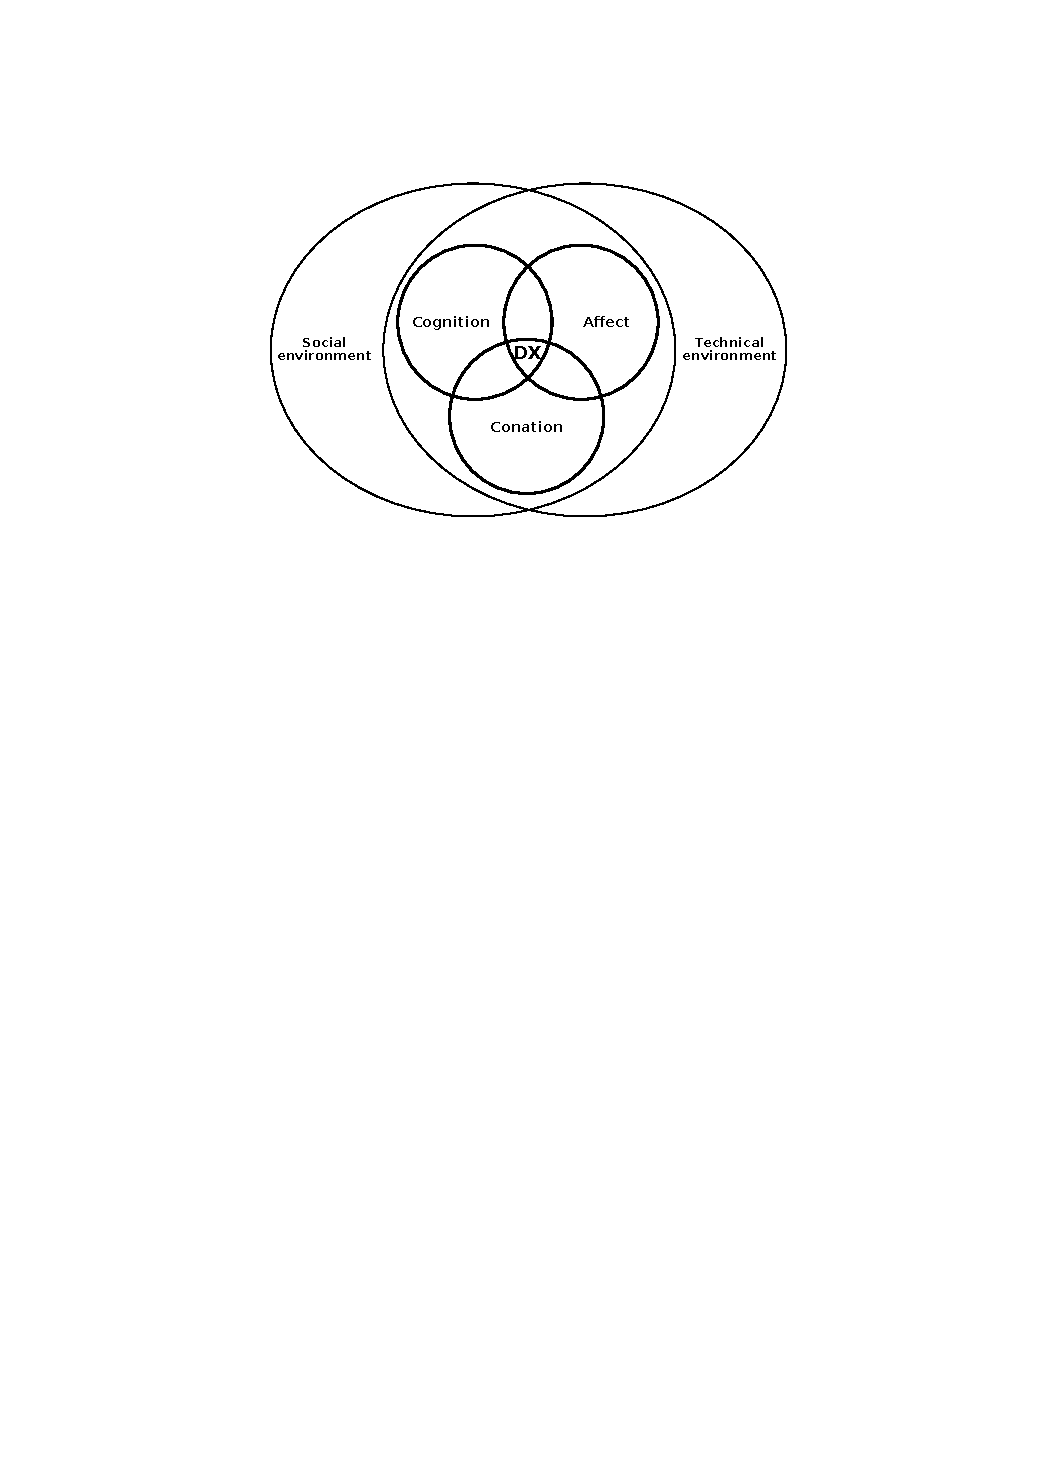
\includegraphics[width=0.6\textwidth]{dx-social-technical.pdf}
  \end{center}
  \label{figure:social-technical}
\end{figure}

\begin{figure}
  \captionsetup{width=0.6\textwidth}
  \caption{Conceptual framework of Developer Experience \citep{fagerholm-dx-concept-and-definition}}
  \begin{center}
    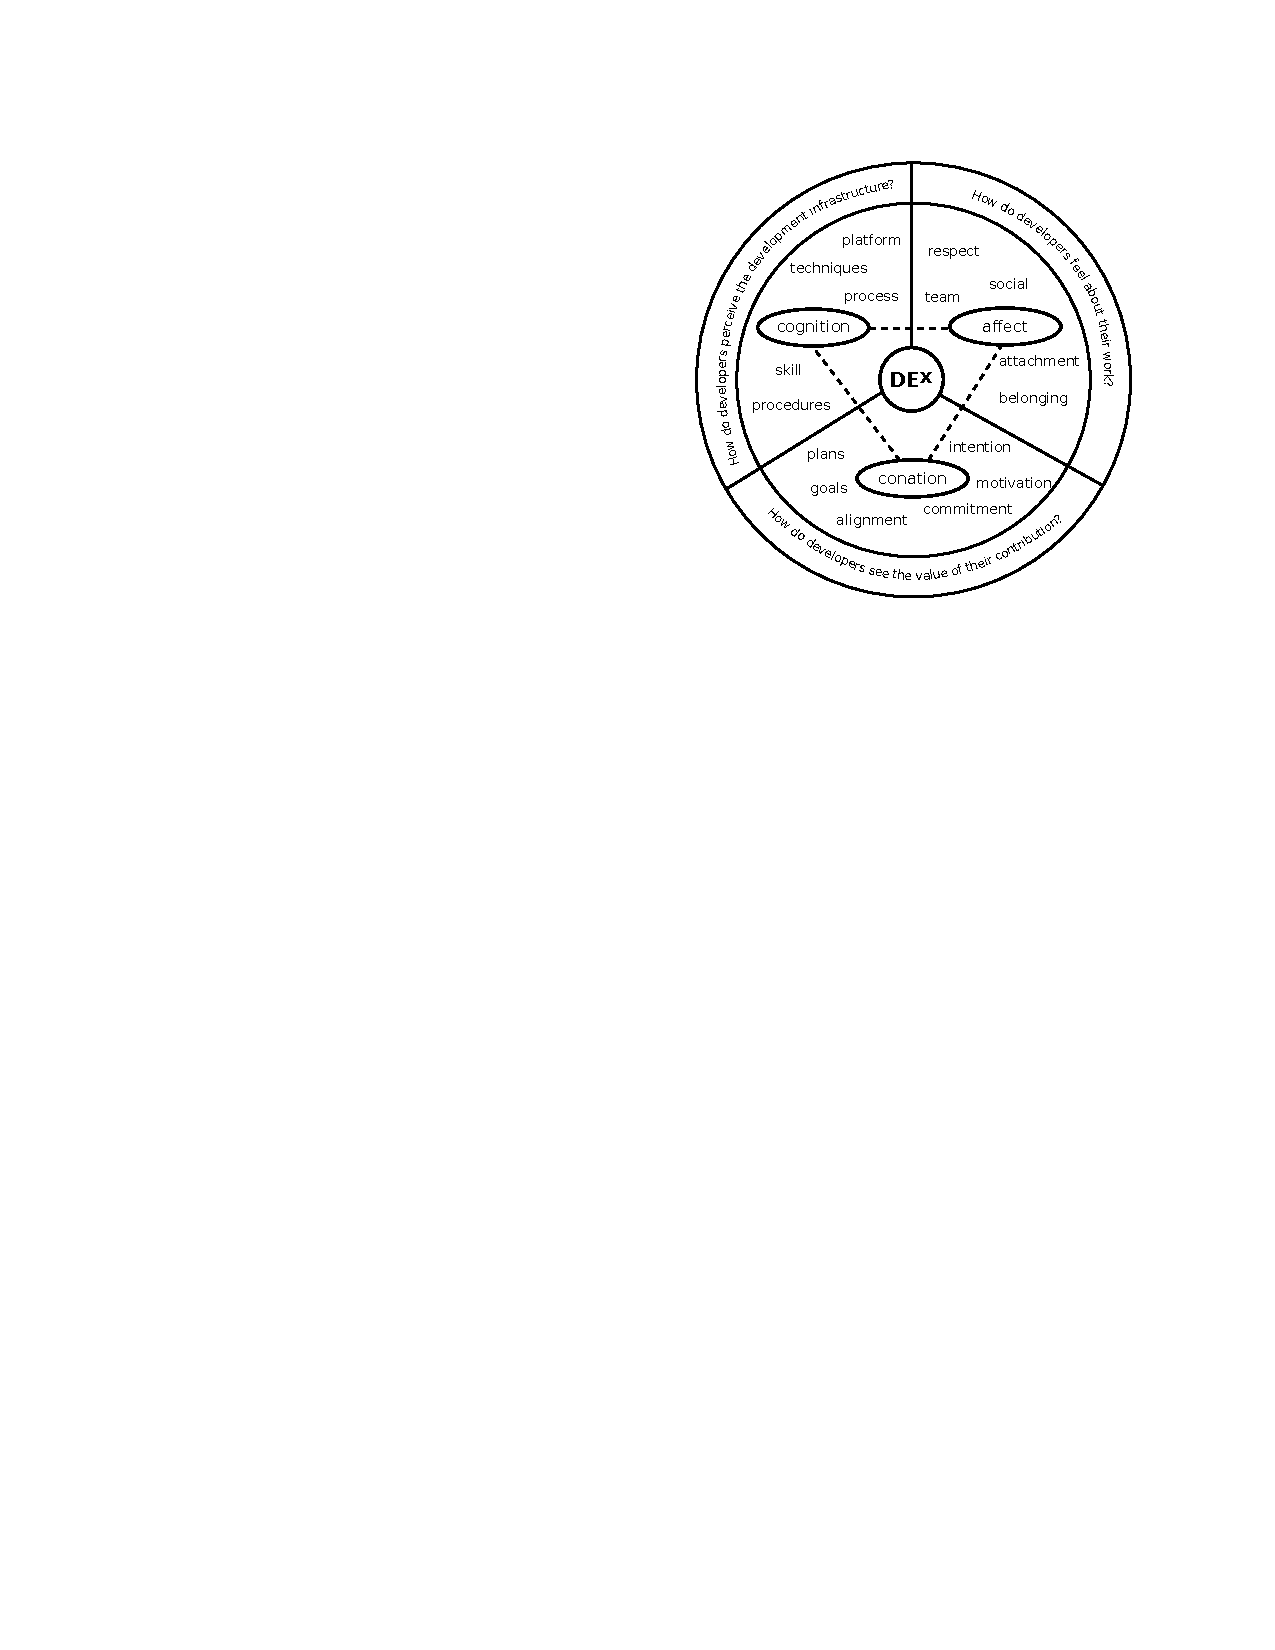
\includegraphics[width=0.6\textwidth]{dx-conceptual.pdf}
  \end{center}
  \label{figure:conceptual-framework}
\end{figure}

\subsection{Programmer Experience}

A software developer is a person with a bigger responsibility than a programmer. If a programmer is following instructions, requirements, and guidelines, the developer is also finding out what the instructions, requirements and guidelines should be and probably also helps in defining them. Therefore DX is also considering more of the surrounding context than what Programmer Experience (PX) is considering.

DX and its related terms have been studied and researched relatively little at the moment of writing (\now). \cite{programmer-experience} performed a literature review of the term \textit{"Programmer Experience"}, that studied 73 articles that matched their defined search criteria. The study concluded that there is still some ambiguity in the term \textit{Programmer Experience} in the context of programming environments, design documents, and programming codes.

Developer Experience (DX) is a bigger construct than PX. DX includes also the motivation of developers, and not only the artefacts like the programming environments \citep{programmer-experience}. Developer Experience is considering also the social aspect of being a software developer. Developer Experience is what is felt by the developer while trying to achieve a goal i.e. completing a project

Programmer Experience (PX) can be defined as \textit{The result of the intrinsic motivations and perceptions of programmers about the use of development artifacts} \citep{programmer-experience}. A programmer can be seen as person who gives exact instructions on how a program should behave and function. PX is based on the study mainly related to the programming environment, but also programming codes and Application Programming Interfaces (API).

% http://programming-experience.org/px19/ https://2019.programming-conference.org/

\subsection{Selection of tools}

Perceived choice is a perception of that the choice has already been made \citep{flow-intrinsic-dx}. Selecting tools in software development projects is in a crucial role, as it can significantly improve the Developer Experience in software projects.

\cite{flow-intrinsic-dx} studied Integrated Development Environment (IDE), and how they are connected with state of flow, intrinsic motivation, and user experience. Their findings reveal that if the developers have a high perception of choice, the also are overall more satisfied with the tools. They also concluded that if the selected tools are selected without their input, (they perceive it chosen already), the developers will have a worse developer experience with it, as e.g. their frustration with the tool will be more common.

There has been a study on the Developer Experience of IDEs \citep{software-developers-as-users}. However, the study concentrated on the UX of the selected IDE that was studied.

When selecting an IDE it is also important to consider what the other developers in the team or organization is using or what other would prefer to use.

\cite{design-framework-enchancing}

There can be situations when two different developers use a different IDE, and therefore also the experience can be completely different between them. At the most extreme the 2 IDEs are not compatible with each other as their files related to the project are different. An example of this is Eclipse and IntelliJ IDEA as Java IDEs.

In a study of IDEs \citep{software-developers-as-users}, the survey in the study produced answers that were most pragmatic, but not hedonic. This could show that most of the developers are practical, and not feeling based. This has also been proven \citep{personality-software}. This might also be a reason why Developer Experience has not gotten that much attention yet, as big part of people in software engineering are \textit{"Introverts"}. Software engineers are also more logical thinkers than feeling based. As Developer Experience is focusing on the feelings and subjective opinions about things, it might be a difficult topic to research.

\subsection{Organization and project onboarding}

\cite{entering-an-ecosystem} have studied the process of entering an ecosystem from the perspective of developers. They have especially focused on the onboarding process of Hybrid Open Source Software projects that have special characteristics as software projects.

Open Source Software (OSS) is software developed, where the source code of the software is accessible to the public. OSS is often developed by a community where anyone participating is allowed to report problems, suggest changes, and also modify the code and develop the software. However, the fact that anyone interested can participate in the community results in that the communities often create their own complex organization and hierarchy.

A hybrid OSS can consist of individual developers, but also sponsored and supported developers that are pursuing the interests of some other organization. One example of this is JavaScript framework React, that was initially developed at Facebook, but later open sourced. Hybrid OSS creates another layer of complexity of the organization.

\cite{entering-an-ecosystem} argue that onboarding and welcoming new developers to hybrid OSS might be more difficult than normal OSS projects. All in all, onboarding of any kind of software project is part of the whole DX of the onboarding developer.

\subsection{Motivation}

Intrinsic Motivation (IM) is the motivation that is enabled by someone enjoying their own work, i.e. the motivation is originating from the work itself. Extrinsic Motivation (EM) is motivation that stems from the outcomes of the work performed \citep{flow-intrinsic-dx} (Self-determination theory. Handbook of theories of social psychology).

\subsection{Performance Alignment Work}

\cite{how-developers-experience-team-performance} and \cite{paw} have created a framework called Performance Alignment Work (PAW), that explains the phenomena of experiencing performance in software development context. Software development performance is a complex construct where performance measurement is not a straightforward practice.

The PAW framework acknowledges that performance can not be measured trough some objective measures, as there are too many different viewpoints to measure software project performance from. It also acknowledges that performance exists on multiple different levels e.g. individual, team, organization, or customer level. Their study concluded that high-performing teams are considered high-performing because the are able to alter the ways the performance of the team is measured. 

The performance of a software development project is highly linked with the DX of the individual and the whole team, and \cite{how-developers-experience-team-performance} suggest that by aligning affective and conative aspects with individual developers and within the whole software development team, there could be opportunities to reach improved performance.

\subsection{Happiness of developers}

Happiness of developers has been reported have high impact on the practice of software development and have consequences. A series of studies, namely \cite{unhappy-developers}, \cite{on-the-unhappiness}, \cite{consequences-of-unhappiness}, and \cite{what-happens-when-unhappy} studies the happiness and unhappiness of developers. They concluded that the (un)happiness of the developer has consequences on the themselves, the process, and the end product. The concept of DX \citep{fagerholm-dx-concept-and-definition} includes the affective dimension that is directly related to the happiness of developers.

\subsection{Flow state}

The flow state is a state where the task at hand has gotten full attention \citep{flow-intrinsic-dx}. Flow state is something that many developers want to achieve. For some developers it is really difficult to focus if there are external things that disturb them like sound or something similar. Also, people coming and asking questions might disturb or interrupt the flow state. Therefore many developers are now also trying out remote work where they are not co-located. Achieving flow state requires a clear set of goals, continuous feedback, and a good balance between skills and challenge. 

\subsection{User Starting Experience}

\cite{api-designers} introduce the concepts of \textit{0 to 200} and \textit{Time to Hello World}. These both concepts are discussing the approachability of APIs. Developers have become more and more in charge of the decision and selection of the tools and 3rd party products that are used when developing software. This might have been more of a responsibility of the organization or the directors or managers before. Now however, it has been seen that the developers are the most knowledgeable persons to make these decisions. \cite{api-designers} argue that the first encounter with the API determines if it's selected for usage or not, especially if there is a set of different options to choose from. Therefore they also say that the \textit{0 to 200} and \textit{Time to Hello World} are important things to consider when developing APIs with a good DX.

\textit{0 to 200} comes from the Hypertext Transfer Protocol HTTP code 200 indicating a successful OK response. Adopting a new API and successfully calling the API with a 200 OK response can be seen as the minimal effort to get the integration working. 

\textit{Time to Hello World} comes from the introduction and adoption a new programming language, where often the first task is to print or log the string "Hello World" to the console or terminal. Adoting the basic structures and building block of the programming language prove how easy it is to get going with it, and therefore can be a measurement of the approachability of the language. 

However, this shouldn't be limited or restricted to only APIs, programming languages, or frameworks. The concept of User Starting Experience could be used in the measurement of introducing or adopting anything new related to software development e.g. a new development technique or process.  

\clearpage
\section{Research methods}

During the study, the research problem and the research questions evolved as the understanding and comprehension of the problem improved. Because of this the planned research methods and the goals with these also evolved and were reshaped when new information was acquired. From the introduction and motivation in sections \ref{introduction} and \ref{motivation}, it was determined that DX is a novel and abstract construct. The concepts and definitions of it are multiple, and vary both in research and in industry. This means that the author's understanding of the topic improved and evolved during the study.

\cite{easterbrook2008selecting} define a set of guidelines for empirical research in software engineering. They argue that selecting a clear research question, an explicit philosophical stance, and an appropriate research method are key when researching in the context of Software Engineering (SE). They also note that many research projects in SE fail in defining the stance of the research, which then further complicates all aspects of the research including its interpretation, validity, replicability etc.

During writing of the thesis, the author was working at the case company, allowing to perform ethnographic techniques in understanding and studying the phenomena. Working at the case company also allowed to have discussion with colleagues.

\subsection{Research approach}

This thesis takes an exploratory approach to study the research problem and to answer the research questions. A research with an exploratory approach considers questions that address the existence of a phenomena, try to describe something \citep{easterbrook2008selecting}. The definition of DX given by \cite{fagerholm-dx-concept-and-definition} will work as the basis of the study, but it is only giving the abstract concept to build upon. This concept and framework has not widely been taken into practice into empirical research.

Also, from initial discussion in the case company there was almost as many definitions of DX as there was discussions. This shows that depending on the role of the practitioner and the context they are working in affects in the definition of DX.

\subsection{Research philosophy}

According to \cite{easterbrook2008selecting}, making explicit decisions on the research methods is key, and by doing that the research becomes more beneficial for practitioners and other researchers. Therefore they also argue that explicitly defining every step of the research should be done.

This thesis will take a \textbf{constructivism} view of the truth, combined with pragmatic approach. A constructivist approach sees the problem as that the human context is always present, and that it is an important part of the research and the study. The \textbf{pragmatic} approach is also required because of the case company in this study. The context of a company is important to include, as something that works with one company, might not work with another company. The pragmatic approach can be seen as an approach from engineering, where the interest is focused on what works at a specific time in a specific context.

An \textbf{positivism} is not a suitable approach in this context. A positivistic approach tries to build up knowledge on verifiable observations that is then incrementally built upon. Positivists prefer to create specific theories from where testable hypotheses are extracted. These hypotheses are then tested in an controlled and isolated environment \citep{easterbrook2008selecting}.

\subsection{Unit of analysis}

\cite{easterbrook2008selecting} point out that it is important to pick the unit of analysis of the study. The unit in this case could be a company or organization, a project, a team, or an individual software developer. As DX is the experience of an individual developer, it is selected as the primary focus in this study.

Another viewpoint to this is also the case company, that has its own culture and set of practices. This study will also see the company as a unit of analysis. The company culture and practices are something that is shared between every developer and other employees.

\subsection{Research method selection}

To be able to investigate and define the definition of DX at the case company, the study has to focus on the foundations. During early stages of the thesis, it was noted that a comprehensive literature review and study was required. A good literature review gives a good foundation on which to build the research upon, and ensures that the studied field is understood correctly.

\subsubsection{Multivocal Literature Review}

Each research and study should have a background check and literature review where previous material and research is assessed, and from where the current research can be continued from an built upon.

A MLR is a form of systematic literature review, that produces both qualitative and quantitative data. In this study a MLR was seen as a good fit, as it allows to get a broad view of the current state of the research in the topic. It also allows to answer exploratory questions where the existence of a subject or topic is abstract or vague.

A more comprehensive discussion of the MLR is discussed in section \ref{mlr}.

% is this subsection of MLR required here or can it be discussed completely in the section of MLR

\subsubsection{Brainstorming}

Brainstorming (BS) is a widely used technique, where the idea is to foster unique and novel ideas. Usually BS sessions are conducted when there is a need for innovation and new ideas. One typical use case of BS would be in a context of developing a product. With help of involving the development team in a BS session, new ideas and possible development directions can be found. The foundation of BS lies in that there are no right and wrong ideas, and that every idea is welcome.

In the context of this thesis, the technique of BS works as an exploratory way of initiating the study. Because of the novelty of the research topic DX, BS is an appropriate way of establishing the initial understanding of DX in the context of the study and the case company. Because the researcher has created their own understanding of what DX is, it would interfere with the study results if the researcher would participate into the sessions. It would also be problematic if the researcher would introduce the topic before the session, because the would either change or deepen the personal image of DX that the participants at that moment have. This is in line with the exploratory research philosophy described by \cite{ethnographically-informed}. If the initial session would have been for example a workshop facilitated by the researcher, the researcher might have affected the session, and it would not have yielded in the same results as with a BS session.

Brainstorming types can be identified into \textit{Traditional Brainstorming (TBS)}, \textit{Nominal Brainstorming (NBS)}, \textit{Electronic brainstorming (EBS)} \citep{brainstorming-techniques}. \textit{TBS} are verbal brainstorming sessions where the idea is to brainstorm verbally together in a group face-to-face. \textit{NBS} can be seen as individual BS sessions, where each individual does the brainstorming without working together. \textit{EBS} is a way to conduct BS with help of computers, from where each individual can concurrently input their ideas. Meanwhile the participants can see ideas from others. However there is a level of anonymity that defeats some of the problems with TBS and NBS.  All in all, the different types of BS has been studied and their efficiency is dependent on many factors \citep{productivity-loss-in-brainstorming-groups}, \citep{electronic-brainstorming}, \citep{chainstorm}.

There are some problems with brainstorming sessions \citep{electronic-brainstorming} \citep{chainstorm}. \textit{Evaluation apprehension} means that group members might get the feeling of being judged, and therefore they might feel reticent with bringing out their ideas. \textit{Production blocking} might also be a problem, as working in groups will require everyone to talk on their own turns, which might lead to ideas becoming irrelevant, ideas might be forgot, the ideas might be rehearsed that blocks the generation of new ideas. \textit{Free riding} can also happen when some BS group members rely on other members to perform the BS actions. According to \cite{six-issues-of-brainstorming}, the proponents of brainstorming is the practitioners, and the opponents are often researchers.

In this study the initial brainstorming session was selected to be a combination of TBS and NBS. NBS allows everyone to work individually. The case company has also established itself as working very agile, and therefore mentioned problems with BS do not require any extra actions to mitigate them. The BS session used Think-Pair-Share method \citep{think-pair-share}, where each participant of the session first thinks about the problem and possible ideas by themselves, then after that each individual is paired together where they share their own initial ideas, discard duplicate ideas, and further develop new ideas after the discussion. After pairing, each pair presents their ideas and findings to the whole group.

\subsubsection{Interviews}

Interviews can be conducted with the concept and framework of developer experience, even without having the participants being aware of the definition of Developer Experience. By using the conation, affection, and cognition, it is possible to initiate discussions of the different elements of DX.

% Write a lot more about interviews
% Topics to address:
% - What is the goal of the interviews? 
% - What data is going to be collected from the interviews
% - Semi-structured interviews or some other research approach for the interviews?

\subsection{Timeline}

Mixed-methods approaches are more complex research strategies where multiple different approaches of an empirical study is combined \citep{easterbrook2008selecting}. In mixed-methods approaches the limitations of the different methods are acknowledged, and the limitations of them are mitigated.

\textit{Sequential exploratory strategy} is one specific mixed-methods research approach. In this approach first qualitative data is collected and analyzed, after which the focus shifts towards quantitative data. Purpose of this approach is to first explore the topic with help of qualitative research, and then possibly test some emerging theory with help of quantitative research. Another reason might be to help in interpreting the qualitative data.

\textit{Concurrent triangulation strategy} is another specific approach of mixed-methods \citep{easterbrook2008selecting}, where different research methods are used concurrently. The concurrent research enables to use results from one method to another, and vice versa. This enables to cross-validate research findings.

In this thesis both \textit{sequential exploratory strategy} and \textit{concurrent triangulation strategy} was used as research approaches. The sequential exploratory strategy was implemented by first conducting the initial multivocal and traditional literature reviews, and then only after that the ideation and planning of the workshops started. However at this point the MLR was not finalized, and still had some open questions, and ongoing interpretations and analysis.

The technique of concurrent triangulation strategy was utilized by conducting the MLR and the brainstorming concurrently. While the first iteration of the MLR was being performed, the initial workshop at the case software consultancy company was held. The idea behind a concurrent research was to get as comprehensive definition of the research problem as possible from as many different viewpoints and contexts as possible.

The initiation of the thesis started during the summer of 2019. The topic of the thesis was selected, and the initial and the preliminary research question and problem were defined. At that moment, the concept of DX was too vague to the author. After some discussions and studies on the topic, it was decided that the MLR should be taken as the first step of the study. When the MLR had been initiated the first results from it emerged, at the meantime the context of the empirical study started also to get defined.

\subsection{Analysis of data}

\cite{analyzing-qualitative-data} give a set of guidelines and practices on analysing qualitative data. They state that using qualitative data in research requires discipline, creativity, but also a systematic approach. The divide the analysis of qualitative data into 5 different step: get to know your data, focus the analysis, categorize information, identify patterns and connections within and between categories, and finllay interpretation. Categorization of the data is explained more in the specific sections where categorization, theming, or coding of data is performed. 

\clearpage
\section{Multivocal literature review} \label{mlr}

Traditionally, in SLRs the reviewed literature consists only of literature that is formally published, and thats motivation of publishing is the publication in itself, e.g. publications in journals and conferences. Material that is produced with commercial interests and informally published material and publications are not considered in SLR \citep{guidelines-for-MLR}.

MLRs, are a way to include grey literature into SLRs \citep{the-need-for-MLR}. Grey literature can be defined in different ways, and research fields define grey literature in ways that are meaningful to that specific field.

\begin{quotation}
  \textit{"Grey literature stands for manifold document types produced on all levels of government, academics, business and industry in print and electronic formats that are protected by intellectual property rights, of sufficient quality to be collected and preserved by library holdings or institutional repositories, but not controlled by commercial publishers i.e., where publishing is not the primary activity of the producing body."} \citep{towards-a-prague-definition-of-grey-literature}
\end{quotation}

The Prague Definition of grey literature is strict and therefore not allowing e.g. blog posts to be used on MLRs. However, a specific guideline for including grey literature in literature reviews has been created \citep{guidelines-for-MLR}. This guideline is based on the guidelines on how to perform SLR in SE \citep{guidelines-for-SLR-in-SE}.


\subsection{The motivation behind a MLR}

DX is a complicated subject and topic, and a clear and well defined definition of it does not exist at the moment of writing (August 2019). There is a need to create an understanding of the definition of DX and a basis to build the rest of the thesis upon. Normal literature reviews can help in these cases, and they create a common understanding of the topic that is going to be discussed. However, normal literature reviews are prone to be biased. To avoid bias of the author, and because DX is a subjective concept of the developer, the definition of DX can be reviewed with a help of a Systematic Literature Review (SLR). Systematic literature reviews are a way of producing evidence based results, and they are effective in complex and opinion based fields where a common agreement of a concept or topic might be difficult to find.

In software engineering practitioners constantly produce valuable literature in e.g. technical reports or blog posts, but this material is not considered in SLRs. This has been identified as a problem, and there's been a call for MLRs in SE \citep{the-need-for-MLR}.

An SLR would include only the scientific papers, and therefore it might not be sufficient to only focus on that. In a MLR the GL should provide a current perspective and fill in the gaps of scientific and formal literature \citep{guidelines-for-MLR}.

SE practitioners are producing a lot of literature, that would not be considered in normal literature reviews or SLR. This GL can provide insights about the field of SE, and especially about DX.

A SLR has been conducted on the concept \textit{Programmer Experience} \citep{programmer-experience}. This SLR will be used to guide this MLR.

% Read \citep{guidelines-for-MLR} again after reading \citep{guidelines-for-SLR-in-SE}.

\subsection{The review protocol of the MLR}

DX is a novel concept, and therefore there has been little formal research on the topic. Based on the different levels of literature, white, grey, and black \citep{guidelines-for-MLR} (find correct reference), DX could be seen even to be in the category of black literature.

\newcommand{\mlrdxlink}{https://docs.google.com/spreadsheets/d/1BLX4eQypAvxd3Gzft0s0rqUHdMYaKxPAbpZZ4dAvJqU/edit?usp=sharing}

All data of the MLR can be found \href{\mlrdxlink}{\textbf{here}}. The data collection is done with Google Sheets and is based on the example shown in \citep{guidelines-for-MLR}.

\subsubsection{Research questions}

The foundation for the MLR is the first research question \hyperref[RQ1]{RQ1} (\rqone). The goal is to create a definition of \textit{Developer Experience} with help of both white literature and grey literature.

\subsubsection{Search process}

The search is performed as a manual search by the author from various libraries to gather the academic literature. For grey literature, the Google search engine (https://www.google.com) will be used. To limit the amount of grey literature, only the first 2 pages of searches from google.com will be included. Only 91 percent of participants in a study went to the second page of google results page \citep{google-search}. Therefore it's appropriate to include only the most relevant results from the google search.

\begin{table}[H]
  \begin{tabular}{ l l }
    IEEExplore    & (https://ieeexplore.ieee.org/Xplore/home.jsp)          \\
    ACM           & (https://dl.acm.org/)                                  \\
    ScienceDirect & (https://www.sciencedirect.com/)                       \\
    Scopus        & (https://www.scopus.com/search/form.uri?display=basic)
  \end{tabular}
  \caption{Scientific literature sources for the MLR}
\end{table}

Other possible libraries and sources for resources could have been the following sources:
\begin{itemize}
  \item [--] Google Scholar (https://scholar.google.com)
  \item [--] Citeseer (https://citeseerx.ist.psu.edu/index)
  \item [--] and SpringerLink (https://link.springer.com/)
\end{itemize}

However, they do not provide advanced search with the author keyword as a search criteria.

Search string for both scientific and grey literature will be \textbf{"developer experience"}. Because of an ambiguous definition of DX, only one search string is uses. This assures that all relevant publications are included. Including more words in the search string or creating a more complex search string would require a better understanding of DX, that the author does not have at this moment. Also, including other search strings would bias the search result.

At the moment of writing (August 2019), using "developer experience" as search string produces 3410 results on Google Scholar. On the first round of searching from Google Scholar, the first search with keyword \textbf{"developer experience"} resulted in 2 included papers and 8 excluded. The search keyword needs to be adjusted.

To further narrow down the search, the search was modified to include only results where author keyword was "developer experience". This narrowed down the search significantly, and removed irrelevant results.

Using the author keyword gives results where the author is intentionally discussing the topic. In the case of DX, with searching only with the author keyword, the inclusion/exclusion rate is significantly better than with a full-text search. However, this approach will remove the possibility to discover definitions of DX where the author is not aware of this concept or phenomenon.

\subsubsection{Inclusion criteria}

The material must be in English. Articles that show up in the searches, and that have the words \textbf{developer experience} in consecutive order order are included in the review.

\subsubsection{Exclusion criteria}

Papers that discuss about developer's experience level e.g. \textit{senior} or \textit{junior developer}, will be excluded.

% \subsubsection{Primary study selection process}

\subsubsection{Quality assessment}

Because of the novel topic the quality assessments might not be that crucial in this study.

\subsubsection{Data collection and analysis}

All papers will be collected into one form with the following data points:

\begin{itemize}
  \item The source
  \item Year of publication
  \item Classification of paper
        \begin{itemize}
          \item Type of research
          \item Scope (Research trends or specific research question)
        \end{itemize}
  \item Main software engineering topic area
  \item The author(s) and affiliation (organisation and country)
  \item Research question/issue
  \item Definition of Developer Experience
  \item Point of interest towards Developer Experience (context)
  \item Summary of paper
        %\item Quality score for the study
\end{itemize}

Analysis will be done on the found definitions and concepts of Developer Experience. During the study the collected data points and especially the about developer experience will be refined.

\subsection{Data Collection}

During collection of data different aspects emerged. The process of collection was a continuous refinement of the search method, inclusion and exclusion criteria, data extraction points. During the collection the comprehension and understanding of the base concept of DX was continuously refined.

\subsection{Data Analysis}

The following sections go trough the data points that emerged during the collection of the data

\subsubsection{Definition of DX}

The most common definition of DX in scientific papers is the concept and definition of in  \citep{fagerholm-dx-concept-and-definition}. This definition is at the moment the only stated definition of DX in the formal literature. There is also further derivations on this concept and definition, but nothing that is revolutionizing or that takes another viewpoint.

To analyze how the the definition of DX is given, all articles and papers will be grouped into either having \textbf{implicit} or \textbf{explicit} definition of DX. This division was something that did emerge in the collection and analysis of the material.

\textit{Explicit definition} of DX means that the author has in some words explained or defined the concept of DX, or referenced some other material that gives the definition to it.

\textit{Implicit definition} of DX means that the author doesn't give any definition or explanation of what DX is. The definition can often however be inferred from the context of the paper.

\begin{figure}[H]
  \captionsetup{width=0.6\textwidth}
  \caption{Implicit vs. explicit definition of Developer Experience in scientific literature}
  \begin{center}
    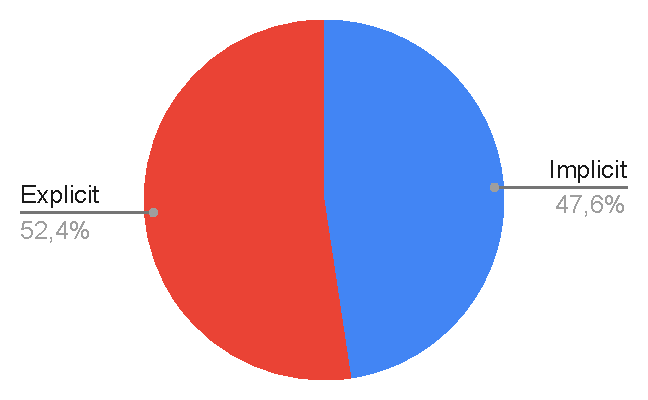
\includegraphics[width=0.6\textwidth]{definition-scientific.pdf}
  \end{center}
\end{figure}

Scientific papers are almost equal in both giving an implicit or explicit definition of DX. It shows and confirms that DX is an topic and research area that has not gotten much attention at the moment of writing. Some research areas have been developed so far that there is things that can be taken for granted. However, the are of DX might not yet be at that point yet and therefore

\begin{figure}[H]
  \captionsetup{width=0.6\textwidth}
  \begin{center}
    \caption{Implicit vs. explicit definition of Developer Experience in grey literature}
    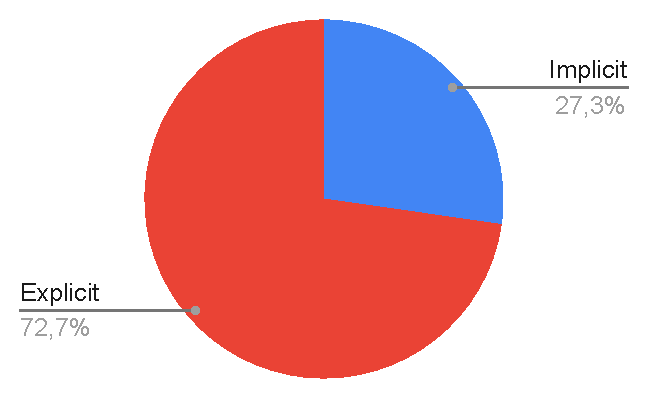
\includegraphics[width=0.6\textwidth]{definition-grey.pdf}
  \end{center}
\end{figure}

Grey literature has a majority of explicit definition of DX. The articles are often starting with giving an explanation of their viewpoint and definition of DX. Quickly the articles then continue to discuss the topic from the selected context and viewpoint.

\subsubsection{Context of DX}

From the analysis of the material, there is a clear indication that there are different viewpoints to DX. The different context that emerged from the analysis are listed in table \ref{table:contexts}.

\begin{table}[H]
  \begin{center}
    \begin{tabular}{l}
      Definition                        \\
      Development Environment           \\
      API                               \\
      Product or service                \\
      User Experience                   \\
      Team, Collaboration, \& Community \\
      Mood \& Feelings                  \\
    \end{tabular}
    \captionsetup{width=0.6\textwidth}
    \caption{Different contexts that emerged during the literature review}
    \label{table:contexts}
  \end{center}
\end{table}

Grey literature takes to a large degree a viewpoint where DX is a form of UX, where developers are users of products and services. In this viewpoint the DX consists of features that are also used when measuring the UX of a service. These include factors like functionality, usability, and reliability.

The grey literature is also heavily influenced by businesses marketing their services or products. To gain visibility and recognition, they are publishing articles and posts on their blogs to write and discuss a specific topic. These businesses are defining DX from their own point of view where they are providing products and services, that are directly used by developers.

Some articles (which?) mentioned that back in the days, it was executives that made the business and purchase decisions of tools, frameworks and other products and the developer's opinion were not considered. Developers were forced to use whatever they were offered.

Today, the purchase decision has more and more shifted to be a responsibility of the developer. Developers are the final users of the product and therefore businesses have probably realized that developers are the ones to make the decisions. All in all, it can be seen from the current grey literature that developers are being considered more and more (Devs are people too), and that this movement has created the concept of DX.

DX allows developers to reason about things that before has been difficult. Making statements that are in the favour of developers might have been difficult as there hasn't been any term to coin the feelings, emotions, needs,

Businesses have taken notice on this movement, and are now utilizing it to create products and services.

DX can be seen that there is always a developer that is a user. The role of the user is the variable, and can vary from being a user of a product where the DX is seen in the product, or then the user can be a user of a developer workflow in a software project.

In many of the grey literature articles the authors have their own view and definition of what DX is. Only in few articles there is actual questioning of the definition of DX.

The formal research on DX has taken a step further and is also considering the social aspects of software development.

A research group in Brazil has to a large extent researched the DX in the context of Mobile Software Ecosystems (MSECO). To these ecosystems belong mobile application development platforms as Android and iOS. Their approach to DX can however be seen as something applicable to all kinds of products and services that aim to create a better DX and improve on it.

Another group of researchers in Finland have studied the mood of developers and its effects at varying levels of software development.

Overall the amount of formal research on DX is lacking. The lack of definitions and the amount of search results in the search speaks for this.


Team, community, and collaboration.


Many articles use the keyword developer experience but only mention DX briefly in their material. This forces the readers to

\begin{table}[H]
  \begin{center}
    \begin{tabular}{l r}
      Definition                        & 5  \\
      Development Environment           & 11 \\
      API                               & 10 \\
      Product or service                & 9  \\
      User Experience                   & 14 \\
      Team, Collaboration, \& Community & 16 \\
      Mood \& Feelings                  & 8  \\
    \end{tabular}
    \caption{Scientific and grey literature combined}
  \end{center}
\end{table}

\begin{table}[H]
  \begin{center}
    \begin{tabular}{l r}
      Definition                        & 4  \\
      Development Environment           & 9  \\
      API                               & 4  \\
      Product or service                & 2  \\
      User Experience                   & 7  \\
      Team, Collaboration, \& Community & 11 \\
      Mood \& Feelings                  & 7  \\
    \end{tabular}
    \caption{Scientific literature}
  \end{center}
\end{table}

\begin{table}[H]
  \begin{center}
    \begin{tabular}{l r}
      Definition                        & 1 \\
      Development Environment           & 2 \\
      API                               & 6 \\
      Product or service                & 7 \\
      User Experience                   & 7 \\
      Team, Collaboration, \& Community & 5 \\
      Mood \& Feelings                  & 1 \\
    \end{tabular}
    \caption{Grey literature}
  \end{center}
\end{table}

\begin{figure}[H]
  \caption{Combined}
  \begin{center}
    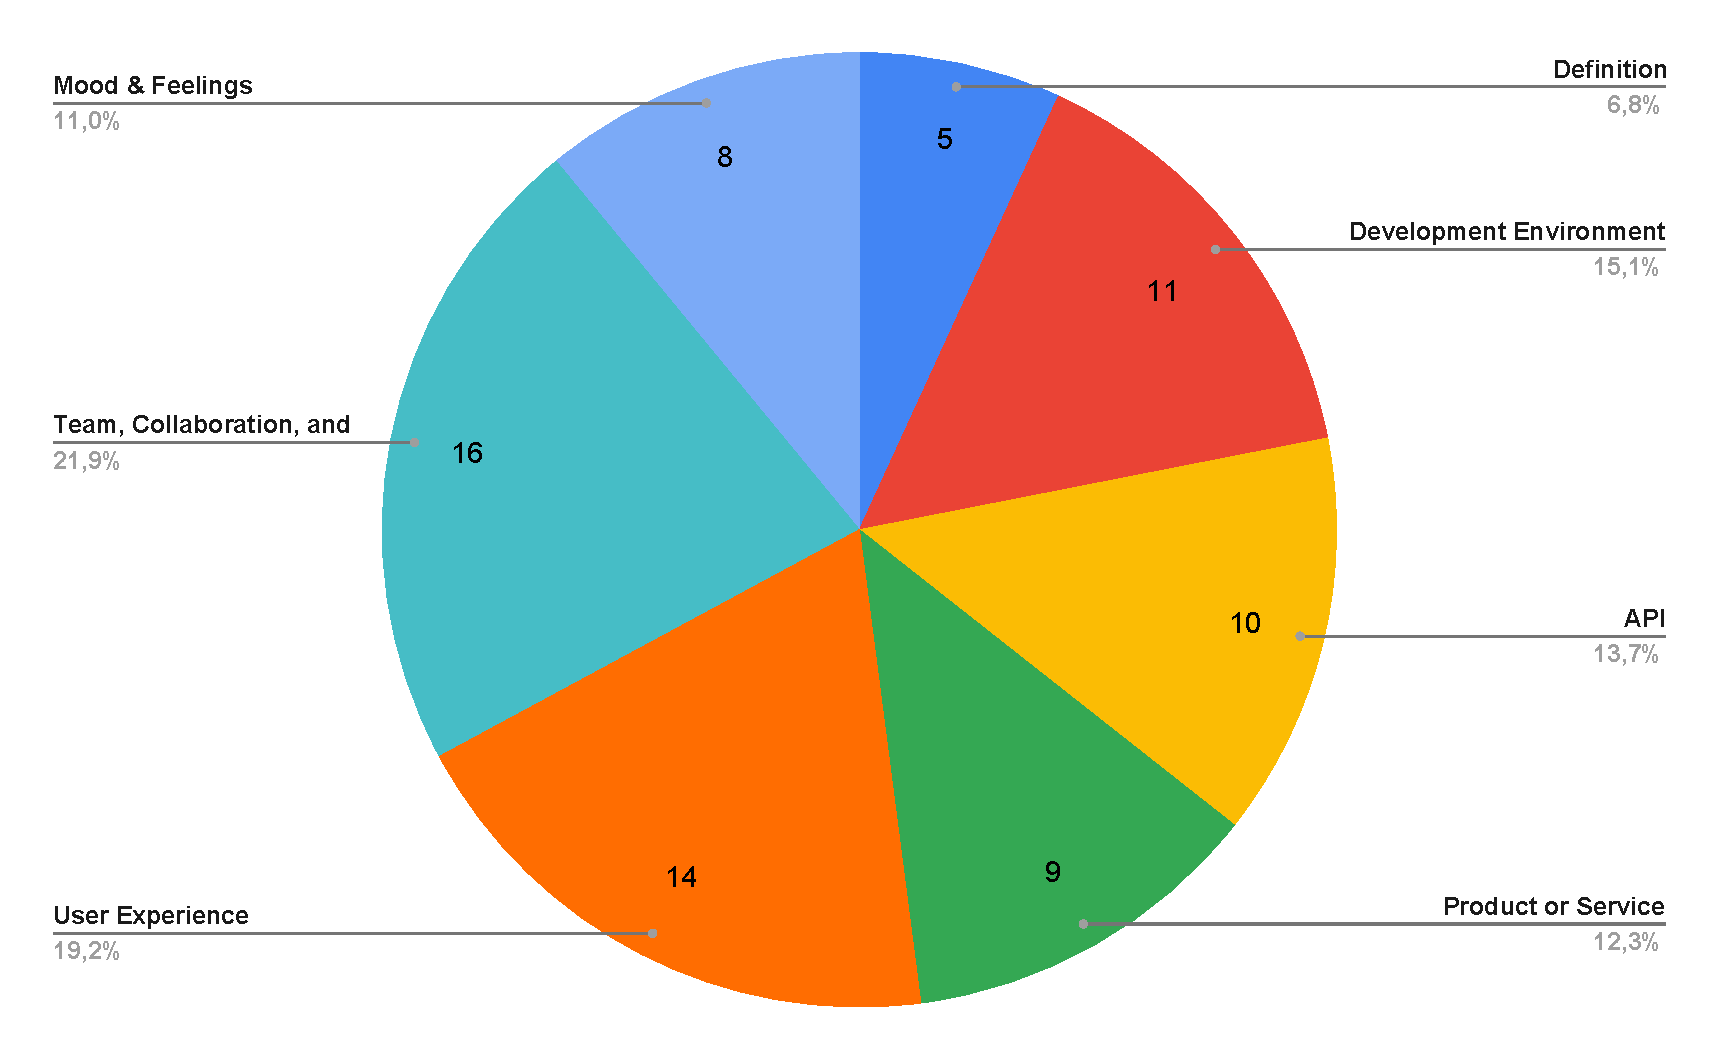
\includegraphics[width=\textwidth]{context-combined.pdf}
  \end{center}
\end{figure}

\begin{figure}[H]
  \caption{Scientific}
  \begin{center}
    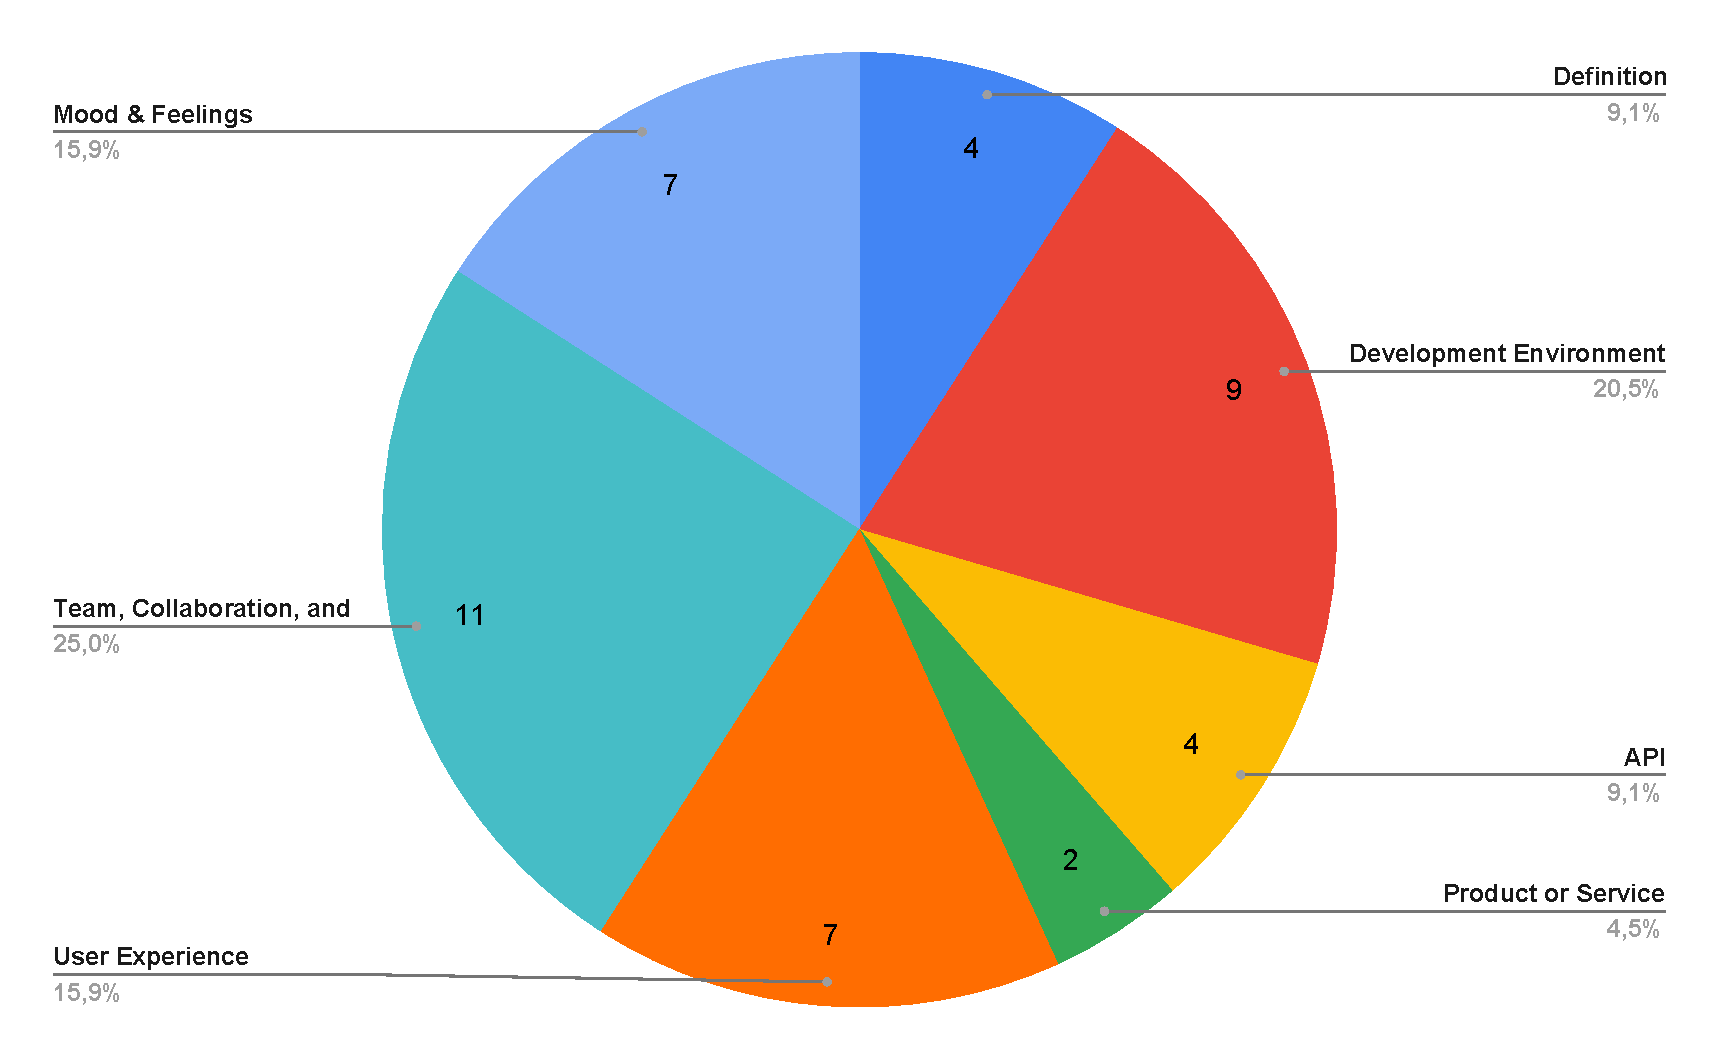
\includegraphics[width=\textwidth]{context-scientific.pdf}
  \end{center}
\end{figure}

\begin{figure}[H]
  \caption{Grey}
  \begin{center}
    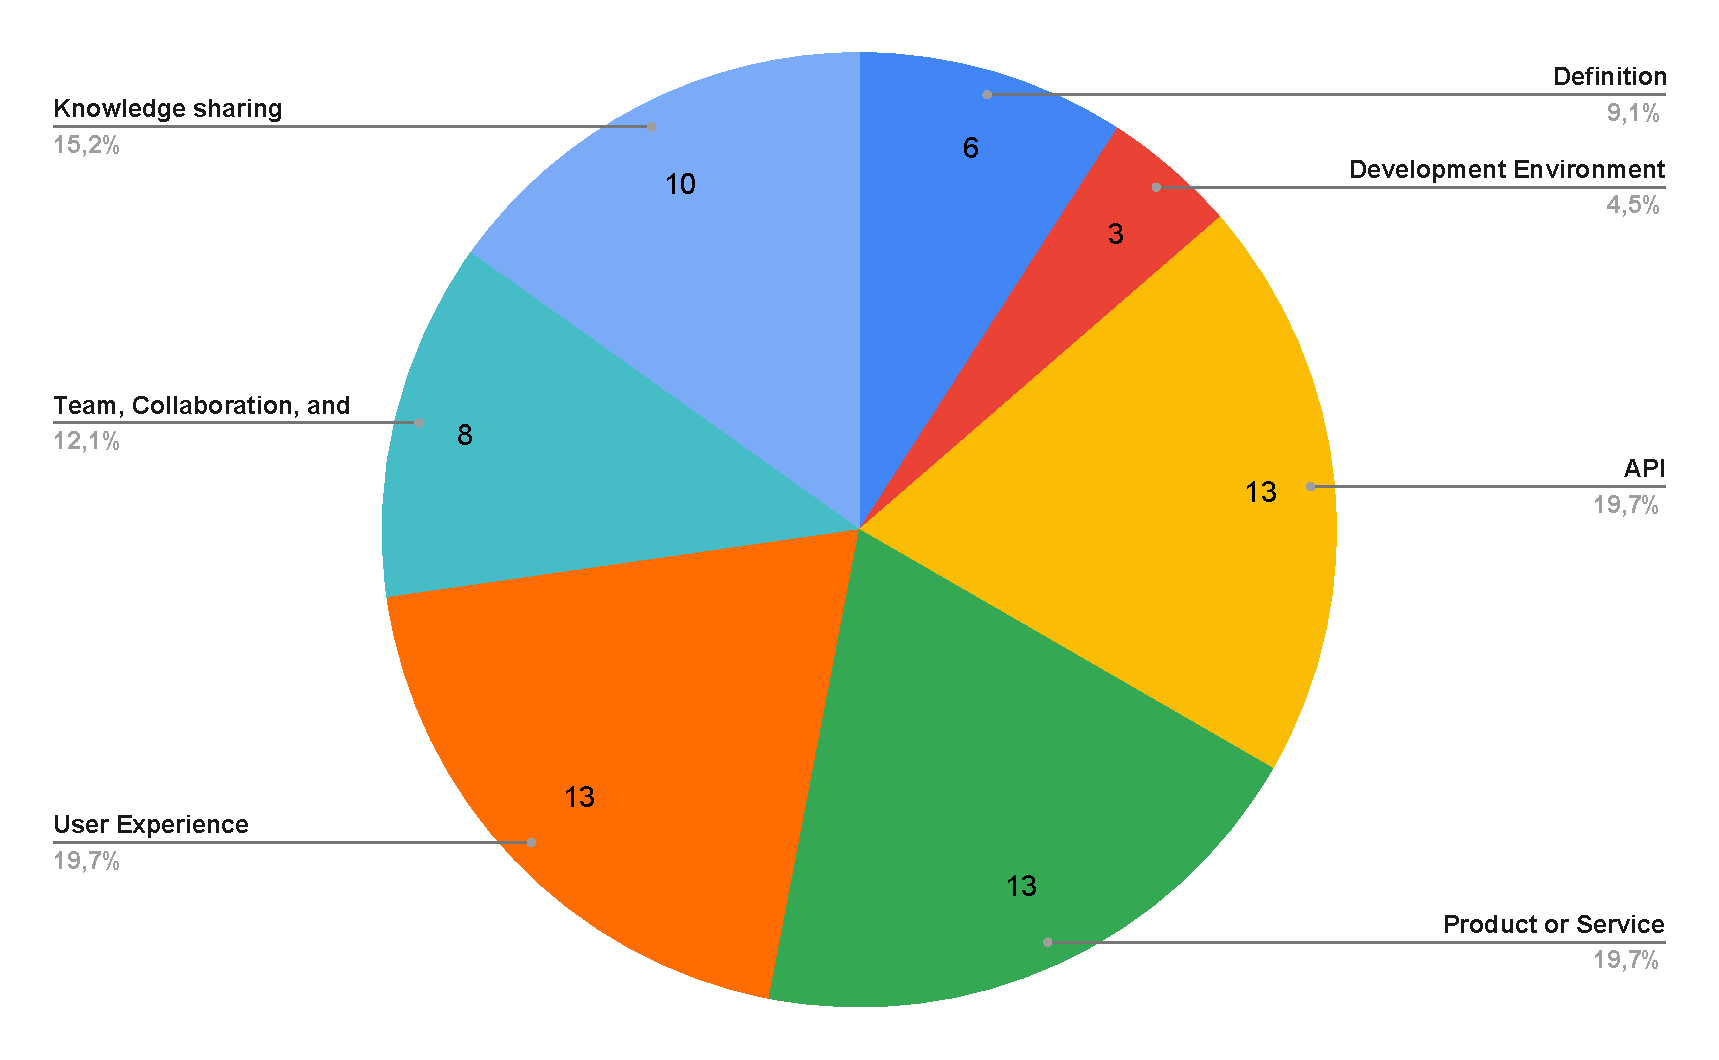
\includegraphics[width=\textwidth]{context-grey.pdf}
  \end{center}
\end{figure}

\subsection{Validity of search results}

The search engine Google is known to provide results based on many different variables on the user e.g. previous searchers, internet profile etc. Therefore the search results from Google might not present results that are applicable for anyone. To mitigate this, private sessions were used when performing the searches.

\clearpage
\section{Current state analysis}


\clearpage
\section{Exploratory research}

Based on the results from the background section and the Multivocal Literature Review, it can be derived that the research topic is complex and difficult to define. Therefore, to gain a better understanding and grasp how DX is thought of in the industry, a workshop and a series of interviews will be conducted.

\textbf{\\ Possible approaches for the practical part of the study:}

\newcommand{\uxdesigndx}{https://uxdesign.cc/contributing-great-developer-experience-designer-e1f497b0fb4}

\begin{itemize}
  \item [--] Based on the \href{\uxdesigndx}{this article}, create a set of guidelines and good practices of DX, and interview and/or measure how well established the application of the practices are
  \item [--] Conduct interviews studying the development environments of different projects. \textit{"When starting a new project, be upfront that you want to tailor your tools and methods for collaboration"}(\href{\uxdesigndx}{uxdesigndx})
  \item [--] Workshop to map current practices and viewpoints on DX
  \item [--] Interviews with individual developers on their viewpoint of DX
\end{itemize}

\subsection{Workshop}

\subsection{Survey (or interviews)}



\clearpage
\section{Results}

Answer the research questions and problem.

\subsection{Validity of results}

T\"ass\"a osassa on syyt\"a my\"os arvioida tutkimustulosten luotettavuutta.
Jos tutkimustulosten merkityst\"a arvioidaan >>Tarkastelu>>-osassa,
voi luotettavuuden arviointi olla my\"os siell\"a.

\clearpage
\section{Summary}

\clearpage
\section{Conclusions}

\clearpage
\thesisbibliography
\bibliography{thesis}

\end{document}
